% Preamble
\documentclass[11pt]{article}

% Packages
\usepackage[spanish]{babel}
\usepackage{graphicx}

\graphicspath{{images}}

\title{Bases de Datos II \\ \large Proyecto Final}
\author{D'Autilio Joel \and Pablo Rossi}

% Document
\begin{document}

       \maketitle
       % \tableofcontents

       \section{Estructura}

       El proyecto consta de tres paquetes principales:

       \begin{itemize}
              \item \textit{structure} contiene clases que representan entidades de una base de datos, como \textit{Table}, \textit{Column} o \textit{Procedure}.
              Un diagrama de este paquete se puede ver en la figura~\ref{fig:uml}
              \item \textit{loader} contiene la clase abstracta \textit{Loader} la cual implementa el método \textit{loadSchema} para cargar el esquema dado en un objeto de tipo \textit{Schema}
              \item \textit{comparator} incluye la clase \textit{DBComparator} que compara dos esquemas y genera un reporte de sus diferencias
       \end{itemize}

       \begin{figure}[ht]
              \centering
              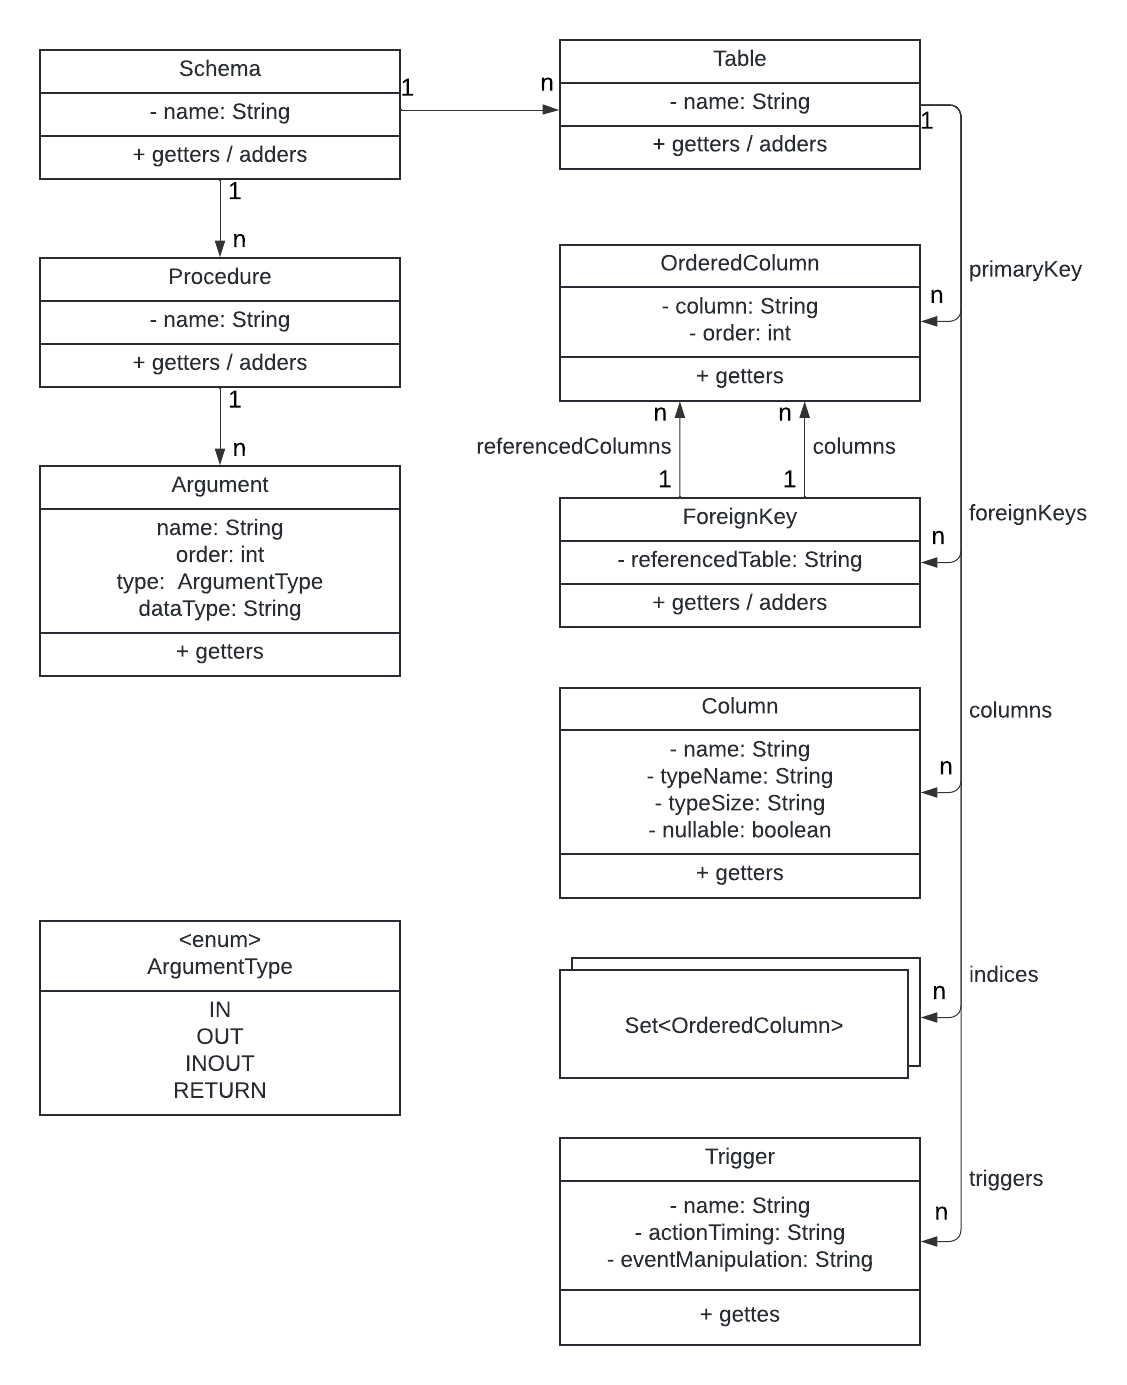
\includegraphics[width=0.9\textwidth]{uml}\label{fig:uml}
              \caption{Diagrama UML de las clases en el paquete \textit{structure}}
       \end{figure}


       \section{Guía de uso}

       El programa se ejecuta en la clase comparator.Main y toma como argumento un archivo de configuración en formato json. Si se pasa un archivo de salida, el reporte se escribe en él. En otro caso, el reporte se escribe en la salida estándar (System.out).

       \subsection{Ejemplos de uso}

       \begin{itemize}
              \item Escribir el reporte en consola
                     \begin{verbatim*}java comparator.Main config.json\end{verbatim*}
              \item Escribir el reporte en el archivo \textit{output.txt}
                     \begin{verbatim*}java comparator.Main config.json -o output.txt\end{verbatim*}
       \end{itemize}


       \section{Lectura de la salida}

\end{document}